\subsubsection{Audio Interfaces}
\label{subsubsec:audio-interfaces}
% Mikrofone und Lautsprecher
% Wie kann ich eigene Dinge abspielen?
% Wo sind /dev/ registriert?
% Was ist installiert? (aplay)
% todo über app wiedergabe

Im Kopf des \gls{go1} ist wie in Abschnitt \ref{par:nano-kopf} beschrieben ein Lautsprecher verbaut.
Ein Blick auf die Hierarchie der verbundenen \gls{usb} Geräte zeigt, dass das Gerät mit der ID \texttt{Dev \num{6}}
die Klasse Audio hat.

\begin{lstlisting}[language=Bash]
unitree@unitree-desktop:~$ lsusb -t | grep Class=Audio
    S|__ Port 4: Dev 6, If 0, Class=Audio, Driver=snd-usb-audio, 12M
    S|__ Port 4: Dev 6, If 1, Class=Audio, Driver=snd-usb-audio, 12M
    S|__ Port 4: Dev 6, If 2, Class=Audio, Driver=snd-usb-audio, 12M
unitree@unitree-desktop:~$ lsusb | grep "Device 006"
Bus 001 Device 006: ID 0d8c:0012 C-Media Electronics, Inc.
\end{lstlisting}

\noindent Der Mount-Point \texttt{/dev/\allowbreak snd/\allowbreak controlC2} des Gerätes lässt sich über den Sym-Link
im Ordner \texttt{/dev/\allowbreak snd/\allowbreak by-id/} auslesen.

\begin{lstlisting}[language=Bash]
unitree@unitree-desktop:~$ ls -l /dev/snd/by-id/
total 0
lrwxrwxrwx 1 root root 12 1x  28 23:58 usb-C-Media_Electronics_Inc._USB_Audio_Device-00 -> ../controlC2
\end{lstlisting}

\noindent Im Folgenden werden zwei Möglichkeiten gezeigt, um den Lautsprecher des Roboters ohne weitere Konfiguration zu nutzen.

\myparagraph{Sprachdurchgabe über App}

Die mobile App für den Roboter ermöglicht es, Mikrofon-Aufnahmen des Gerätes, auf dem die App installiert ist, an den
\gls{go1} zu senden und dann über den Lautsprecher auf der Rückseite des Kopfes abzuspielen.
Hierfür muss die Anwendung zuerst mit dem Roboter verbunden werden.
Danach kann über den Menüpunkt \texttt{Peripherals > Audio Device} auf die Oberfläche zur Konfiguration der Übertragung
zugegriffen werden.
Abbildung \ref{fig:app-audio} zeigt die Übersicht der Audioübertragung.

\begin{figure}[h]
    \frame{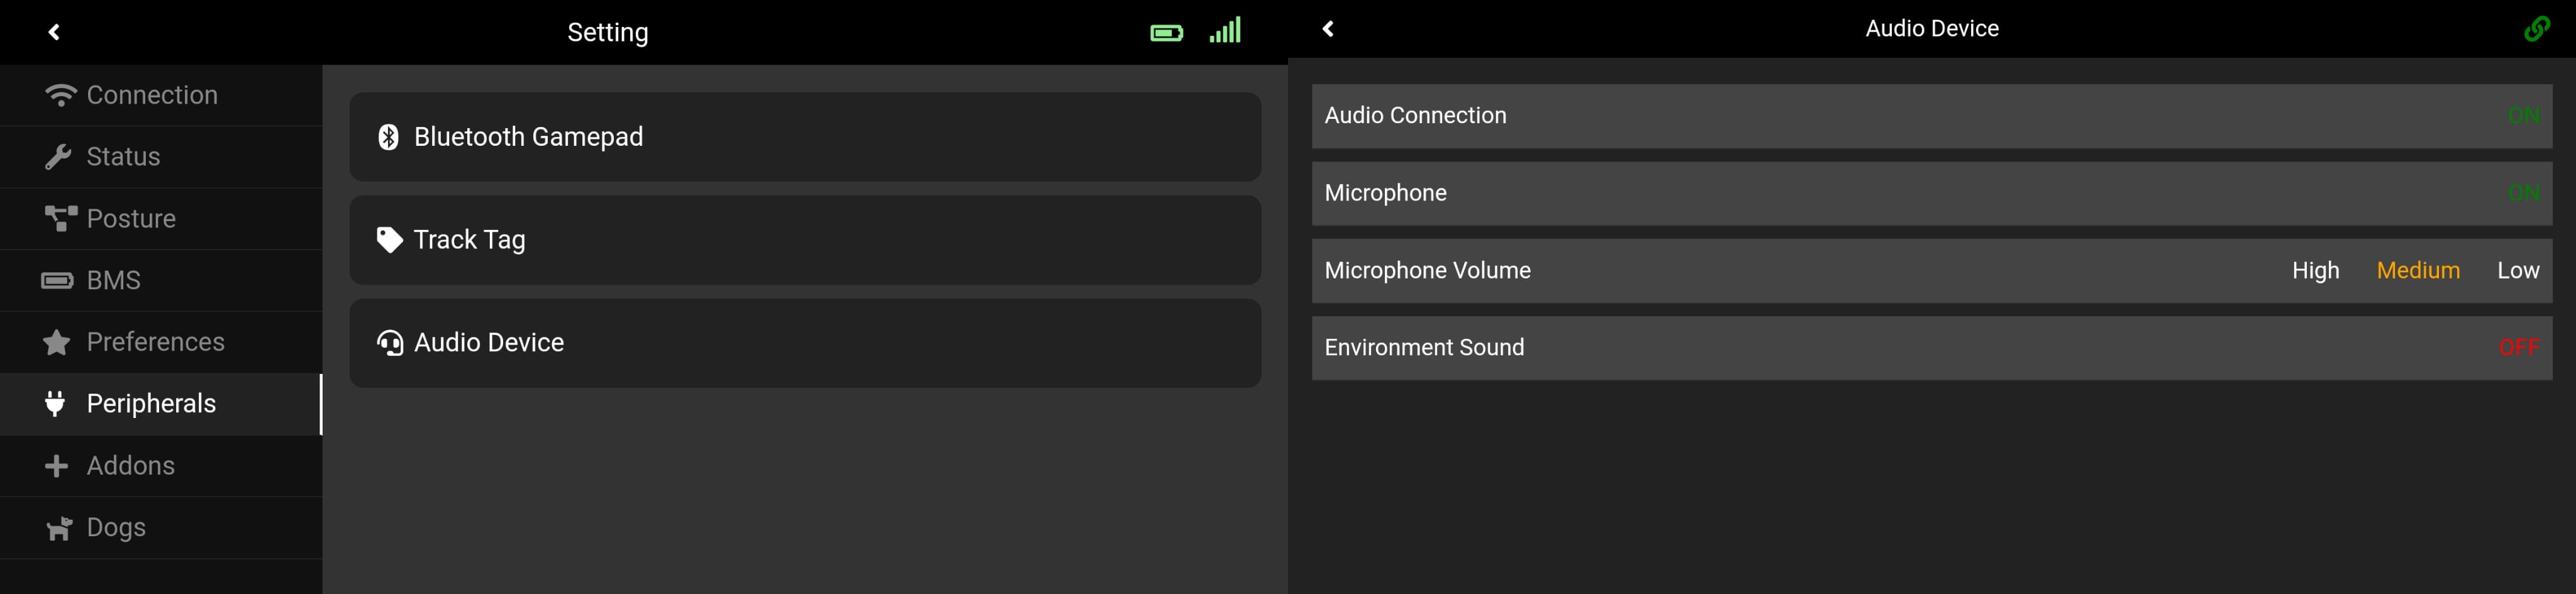
\includegraphics[width=\linewidth]{img/analyse/audio-app}}
    \caption{Überblick über Netzwerkkonfiguration}\label{fig:app-audio}
\end{figure}

Das Icon im rechten oberen Bildrand zeigt an, ob das Audiointerface im Kopf des Hundes erfolgreich verbunden wurde.
Hierfür muss der Autostartprozess \texttt{wsaudio} auf dem Nano noch in Betrieb sein.
Das kann über folgenden Befehl geprüft werden.

\begin{lstlisting}[language=Bash]
unitree@unitree-desktop:~$ ps -aux | grep wsaudio
unitree   8205 95.0  0.4 466312 18360 ?        Rl   00:00   0:23 ./build/wsaudio
\end{lstlisting}

\noindent Sollte dieser Prozess nicht aktiv sein, so kann das Autostartskript manuell ausgeführt werden.

\begin{lstlisting}[language=Bash]
unitree@unitree-desktop:~$ cd /home/unitree/Unitree/autostart/wsaudio/
unitree@unitree-desktop:~/Unitree/autostart/wsaudio$ ./wsaudio.sh &
[1] 9179
[wsaudio] starting ...
unitree@unitree-desktop:~/Unitree/autostart/wsaudio$ ps -ax | grep wsaudio
 9179 pts/0    Rl     3:15 ./build/wsaudio
\end{lstlisting}

\noindent Wichtig ist bei der manuellen Ausführung von Autostartskripten, dass diese aus ihrem Ordner heraus gestartet werden,
da die Skripte selbst oftmals mit relativen Pfaden arbeiten.

In der mobilen Anwendung kann nun der Wert \texttt{Audio Connection} gewählt werden, um diesen von \texttt{OFF} auf
\texttt{ON} zu schalten.
Sobald dies auch für den Wert \texttt{Microphone} erledigt wurde, kann über das eingebaute Mikrofon des Handys, auf dem
die Anwendung läuft, Audio aufgenommen werden.
Das Aufgenommene wird dann mit Netzwerk-bedingter Latenz auf dem Lautsprecher abgespielt.

\myparagraph{Abspielen von Audiodateien}

Für das Abspielen von Audiodateien müssen diese erst auf den Nano im Kopf des Roboters kopiert werden.
Hierfür kann die auf den meisten Linux-basierten Betriebssystemen installierte Funktion \texttt{scp} verwendet werden.
Ist der Rechner mit der Datei im Netzwerk des \gls{go1}, so kann folgender Befehl verwendet werden, um die Datei zu kopieren:

\begin{lstlisting}[language=Bash]
sshpass -p 123 scp beispiel.wav unitree@192.168.123.13:~/Music
\end{lstlisting}

Um den Lautsprecher nutzen zu können, müssen alle Prozesse, die diesen blockieren erst beendet werden.
Ab Werk ist das nur der im vorigen Paragraf beschriebene \texttt{wsaudio}-Prozess, der mit dem Kommando \texttt{pkill -f wsaudio}
beendet werden kann.
Danach kann mit dem Befehl \texttt{aplay} die Datei wiedergegeben werden.
Hierfür wird der Gerätename benötigt, welcher mit dem Befehl \texttt{aplay -L}, in dessen Ausgabe nach dem Gerät mit
der Kennung \num{2} gesucht wird, ausgelesen werden kann.
Die Kennung wurde am Anfang des Kapitels über den Mount-Point erfasst.
Die Ausgabe der Datei \texttt{/proc/\allowbreak asound/\allowbreak cards} zeigt den \gls{usb} Lautsprecher unter dem Index \num{2}.

\begin{lstlisting}[language=Bash]
unitree@unitree-desktop:~$ cat /proc/asound/cards
[...]
 2 [Device         ]: USB-Audio - USB Audio Device
                      C-Media Electronics Inc. USB Audio Device at usb-70090000.xusb-3.4, full speed
\end{lstlisting}

\noindent Die Ausgabe der Datei \texttt{/proc/\allowbreak asound/\allowbreak card2/\allowbreak pcm0p/\allowbreak info}
zeigt, dass die Karte mit dem Index \num{2} nur einen Kanal hat, der für das Abspielen verwendet werden kann
\footnote{\texttt{card2} steht hier für den Index \num{2} der \texttt{/proc/asound/cards}-Liste, \texttt{pcm0p} für das erste \texttt{PLAYBACK} Gerät zur Ausgabe}.

\begin{lstlisting}[language=Bash]
unitree@unitree-desktop:~$ cat /proc/asound/card2/pcm0p/info
card: 2
device: 0
subdevice: 0
stream: PLAYBACK
id: USB Audio
name: USB Audio
subname: subdevice #0
class: 0
subclass: 0
subdevices_count: 1
subdevices_avail: 1
\end{lstlisting}

\noindent Dadurch ergibt sich der direkte Hardwarename des Lautsprechers \texttt{plughw:2,0}
\footnote{\texttt{plug} steht hier für gesteckte Hardware \texttt{hw} (z.B. \gls{usb}), \num{2} für den Index und \num{0} für den Kanal (subdevice)},
welcher für folgenden Befehl benötigt wird:

\begin{lstlisting}[language=Bash]
unitree@unitree-desktop:~$ aplay -D plughw:2,0  ~/Music/beispiel.wav
Playing WAVE '/home/unitree/Music/beispiel.wav' : Signed 16 bit Little Endian, Rate 44100 Hz, Stereo
\end{lstlisting}

\noindent Zur einfacheren Handhabung von einem externen Gerät können auch folgende Befehle verwendet werden, insofern das Gerät mit dem Netzwerk
des \gls{go1} verbunden ist:

\begin{lstlisting}[language=Bash]
sshpass -p 123 ssh unitree@192.168.123.13 'pkill -f wsaudio'
sshpass -p 123 ssh unitree@192.168.123.13 'aplay -D plughw:2,0 ~/Music/beispiel.wav'
\end{lstlisting}

\noindent Um die Lautstärke des Lautsprechers anzupassen, stellt die Bibliothek, die auch \texttt{aplay} enthält, ebenfalls die
Funktion \texttt{amixer} zur Verfügung.
Durch den Befehl \texttt{amixer -c 2 set Speaker <0-100>\%}.
Die Option \texttt{-c 2} verweist hier wieder auf die Gerätekennung.\footcite{alsa}
